\documentclass{beamer}

\usecolortheme{UD}
 
\usepackage{bm}
\usepackage{tikz}
\usetikzlibrary{tikzmark}
\usetikzlibrary{arrows,shapes,backgrounds}
\usepackage{amsmath, amsfonts}

%\usepackage{enumitem}
\usepackage[UKenglish]{babel}
\usepackage{booktabs}
\usepackage{graphicx}
\usepackage{subfig}

\newcommand\DrawBox[6]{% 
	\begin{tikzpicture}[remember picture,overlay]
	\draw[red, ultra thick]([yshift=#3,xshift=#4]pic cs:#1) rectangle ([yshift=#5,xshift=#6]pic cs:#2);
\end{tikzpicture}%
}

\tikzstyle{every picture}+=[remember picture]
\tikzstyle{na} = [baseline=-.5ex]

\setbeamertemplate{itemize items}[circle]

\institute{
\includegraphics[height=1cm]{ud_logo}}

% -----------------------------------------------------------------------------
\graphicspath{ {figs/} }

%Information to be included in the title page:
\title{\bf{Background on Deep Learning}}
\author{Nate Merrill}
\subtitle{University of Delaware}

\begin{document}
 
\frame{\titlepage}


\begin{frame}{Popular Deep Learning Tasks}
        \begin{itemize}
            \item Classification
            \item Classifcation + Bounding Box Detection
            \item Muti-object detection
            \item Pixel-wise semantic segmentation
        \end{itemize}
        \begin{figure}
            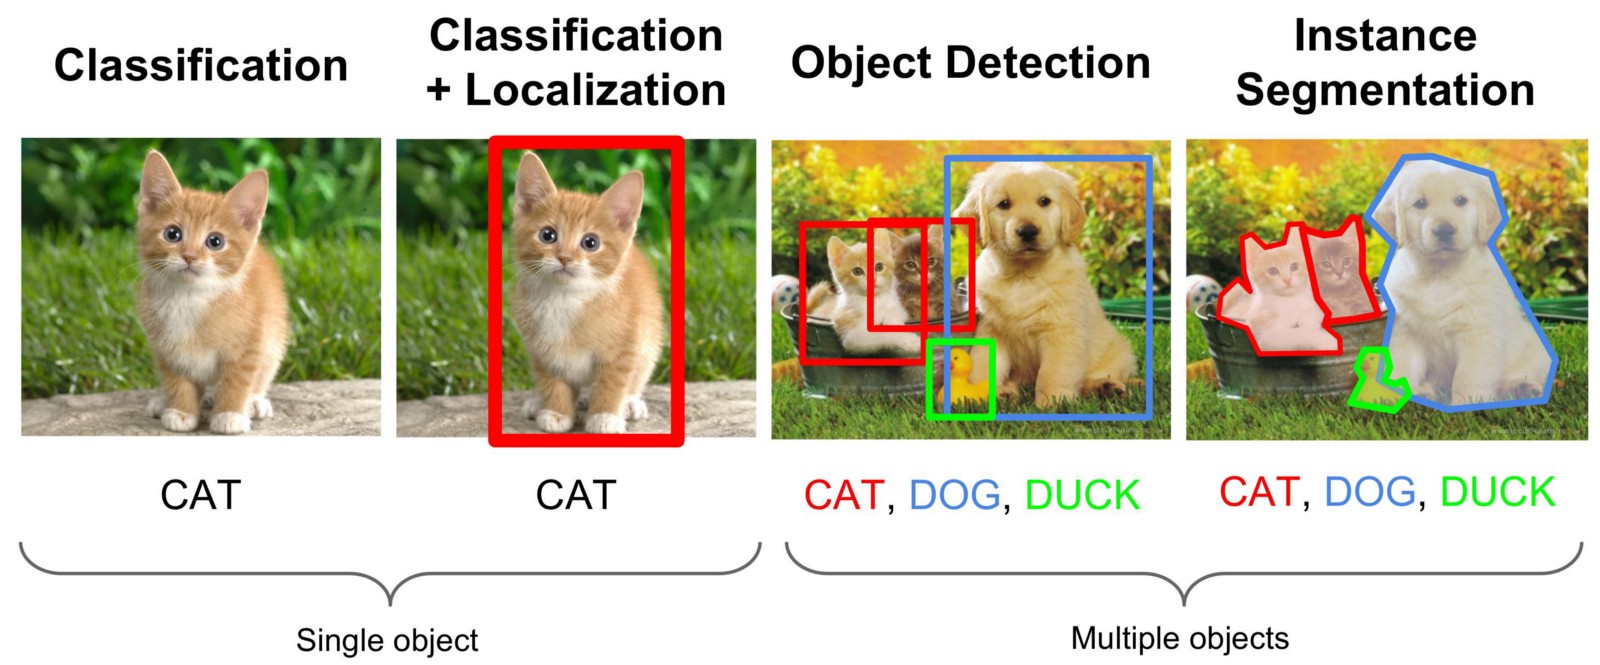
\includegraphics[width=\columnwidth]{kitties}
        \end{figure}
\end{frame}

\begin{frame}{More Popular Deep Learning Tasks}
        \begin{itemize}
            \item Embeddings (dimension reduction)
            \begin{itemize}
                \item Autoencoder
                \item Triplet Embedding
            \end{itemize}
        \end{itemize}
        
        \begin{columns}
            \column{.5\textwidth}
                \begin{figure}
                    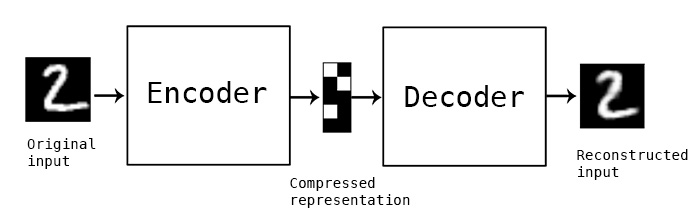
\includegraphics[width=\columnwidth]{autoencoder}
                    \caption*{Autoencoder}
                \end{figure}
            \column{.5\textwidth}
                \begin{figure}
                    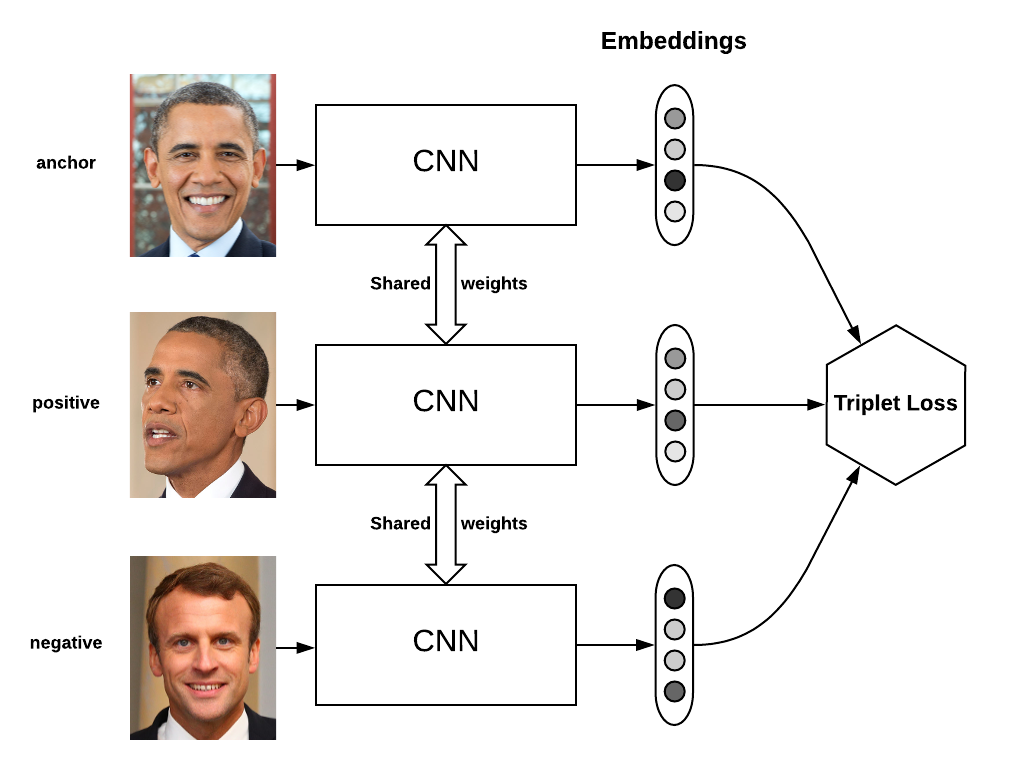
\includegraphics[width=\columnwidth]{triplet_embedding}
                    \caption*{Triplet embedding}
                \end{figure}
        \end{columns}
\end{frame}

\begin{frame}{Fully Connected Layer}
        \begin{columns}
            \column{.5\textwidth}
                \begin{itemize}
                    \item Vector input and output
                    \item Learned weights associated with each connection
                    \item Can be written as a linear operation  
                \end{itemize}
                \vspace{-10pt}
                \begin{align*}
                    \mathbf{x} &= \begin{bmatrix}x_1 & x_2 & \hdots & x_n & 1 \end{bmatrix}^\intercal \\
                     \mathbf{y} &= \begin{bmatrix}y_1 & y_2 & \hdots & y_m \end{bmatrix}^\intercal\\
                     \mathbf{W} &= \begin{bmatrix} w_{11} & w_{12} & \hdots & w_{1n} & b_1 \\
                                                 w_{21} & w_{22} & \hdots & w_{2n} & b_2 \\
                                                 \vdots & \ddots & \ddots & \vdots & \vdots \\
                                                 w_{m1} & w_{m2} & \hdots & w_{mn} & b_m \end{bmatrix} \\ 
                     \mathbf{y} &= \mathbf{W}\mathbf{x}
                \end{align*}

            \column{.5\textwidth}
                \begin{figure}
                    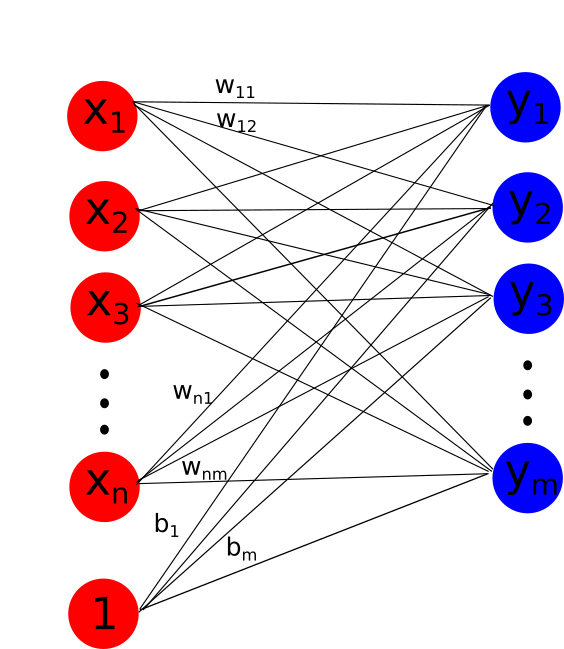
\includegraphics[width=\columnwidth]{fc}
                \end{figure}
        \end{columns}
\end{frame}

\begin{frame}{Nonlinear Activation}
    \begin{itemize}
        \item Fully connected layer cannot model nonlinear functions
        \item Nonlinear activations are used to provide nonlinearity
        \item Key idea: they resemble a "neuron" firing
    \end{itemize}
    Examples:   
    \vspace{-15pt}
    \begin{figure}
        \hspace*{-2cm}
        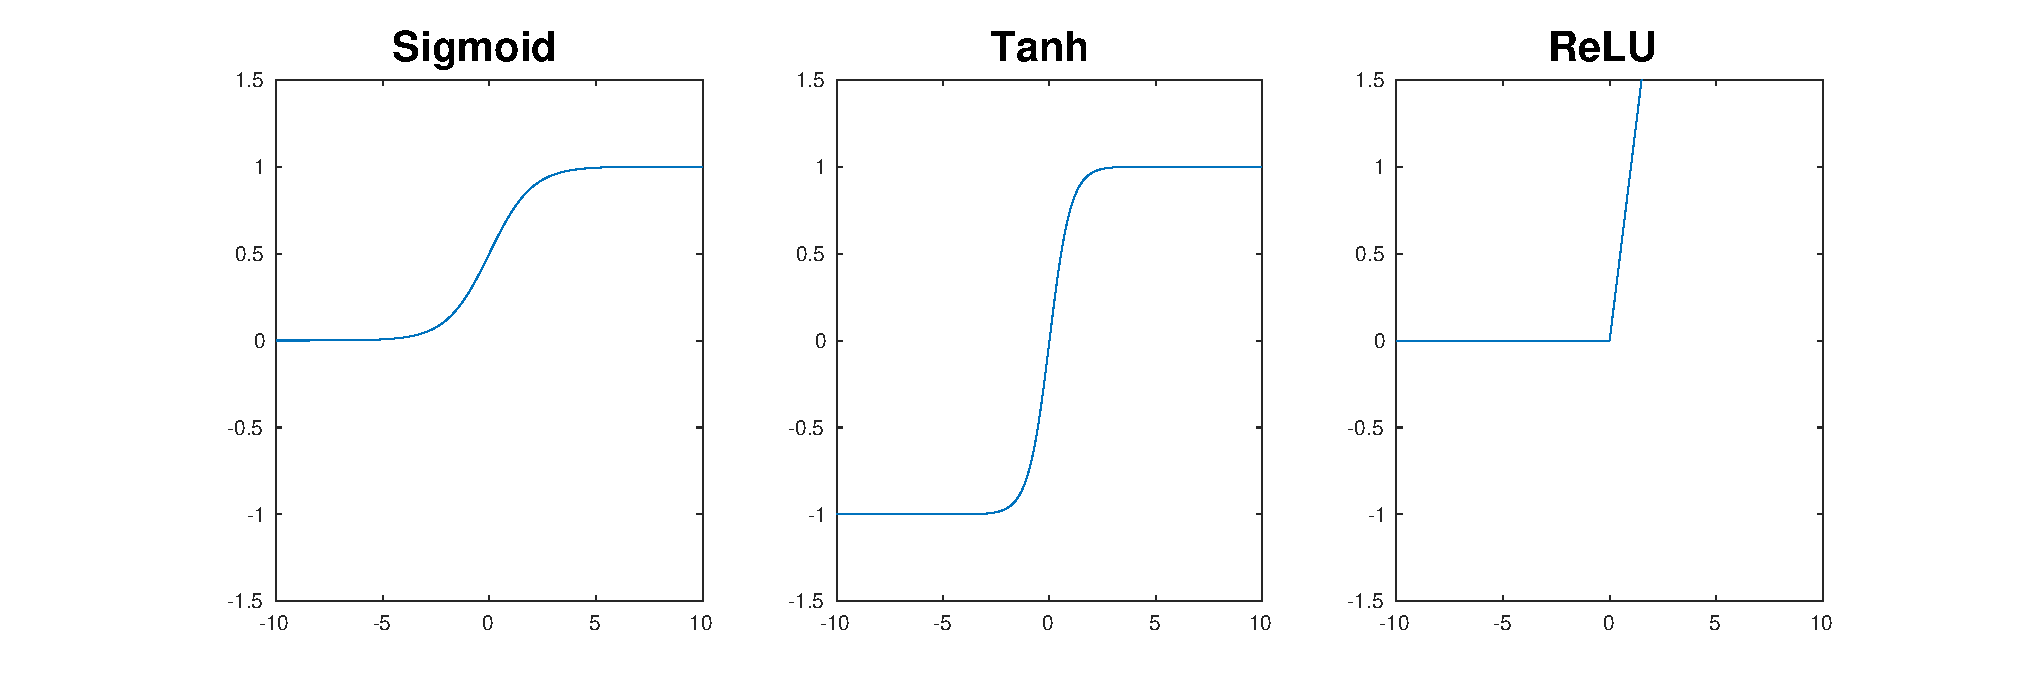
\includegraphics[width=1.33\textwidth]{activations}
        \caption*{Popular activation functions}
    \end{figure}

\end{frame}

\begin{frame}{Convolution Layer}
    \begin{itemize}
        \item Matrix/Tensor input and output
        \item Useful for image input
    \end{itemize}

    \begin{figure}
        \includegraphics[width=\textwidth]{conv}
    \end{figure}

    \vspace{-10pt}
    \begin{align*}
        Y_{ij} =\ & K_{33}X_{i,j} + K_{32}X_{i,j+1} + K_{31}X_{i,j+2} + K_{23}X_{i+1,j} \\
               &  + K_{22}X_{i+1,j+1} + K_{21}X_{i+1,j+2} + K_{13}X_{i+2,j} \\
               & + K_{12}X_{i+2,j+1} + K_{11}X_{i+2,j+2} + b
    \end{align*}
\end{frame}

\begin{frame}{Max Pooling Layer}
    \begin{itemize}
        \item Useful for viewpoint invariance
        \item Similar operation to convolution
    \end{itemize}


    \begin{figure}
        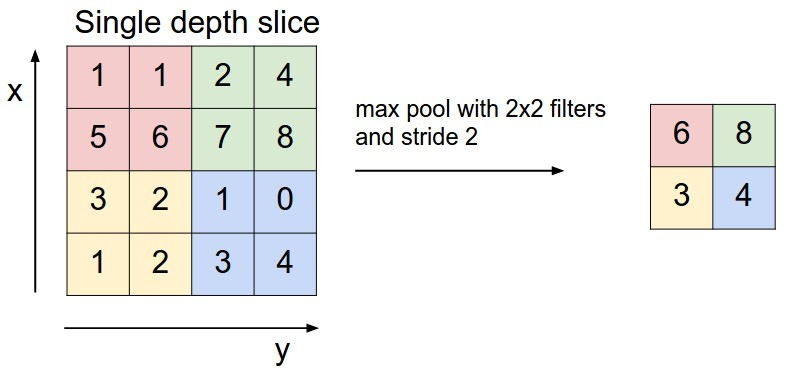
\includegraphics[width=\textwidth]{maxpool}
    \end{figure}
\end{frame}

\begin{frame}{Softmax Layer}
    \begin{itemize}
        \item Bounds output to [0,1]
        \item Sum of output is 1
        \item Useful for learning probability mass functions
    \end{itemize}

    Suppose $\mathbf{x} \in \mathbb{R}^n$, then 

    \[
        Softmax(x_i) = \frac{e^{x_i}}{\sum_{j=1}^{n} e^{x_j}}
    \]

\end{frame}

\begin{frame}{Loss Function}
    \begin{itemize}
        \item A scalar error metric for the network
        \item Necessary for training. Otherwise there is no optimization criteria
    \end{itemize}
    \hspace{-10pt}{\bf Popular examples:}

    \vspace{20pt}
    \begin{columns}
        \column{0.5\textwidth}
            {\bf Cross Entropy}

            Suppose $\mathbf{x} \in \{0,1\}^n$ is the ground truth class labels
            and $\hat{\mathbf{x}} \in [0,1]^n$ is the output of a \textit{classification} network, then
            \[
                E(\mathbf{x}, \hat{\mathbf{x}}) = -\sum_{i=1}^n x_i \ln(\hat{x}_i)
            \]
        \column{0.5\textwidth}
            {\bf MSE}
            Suppose $\mathbf{x} \in \mathbb{R}^n$ is the ground truth  
            and $\hat{\mathbf{x}} \in \mathbb{R}^n$ is the output of a \textit{regression} network, then
            \[
                E(\mathbf{x}, \hat{\mathbf{x}}) = \frac{1}{n} ||\hat{\mathbf{x}} - \mathbf{x}||_2^2
            \]
            \vspace{10pt}

    \end{columns}    

\end{frame}

\begin{frame}{Optimization}

    \begin{itemize}
        \item<1-> Suppose we have a feed-forward neural network with arbitrary tensor input $\bm{X}$, output (loss/error) $E$, and layers $L_1, L_2, \hdots, L_k$ (including loss layer).
        \item<1-> How can we optimize such a complicated function?
        \item<1-> There are many local minimums to get caught in
        \begin{itemize}
            \item<2-> {\bf Idea:} Look at each layer separately
            \item<2-> Observe that $E = L_k(L_{k-1} (\hdots (L_1(\bm{X}))))$.
            \item<2-> We can estimate the gradient of the entire network with the chain rule!
        \end{itemize}
    \end{itemize}

    \begin{figure}
        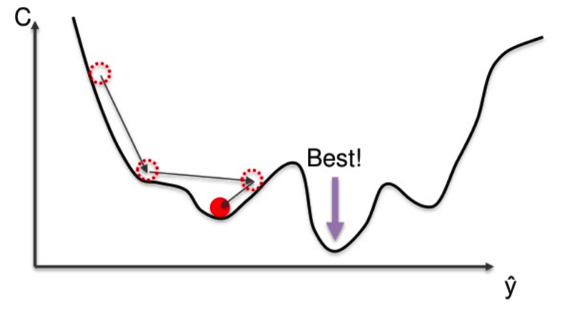
\includegraphics[width=.5\textwidth]{minimum}
    \end{figure}
\end{frame}

\begin{frame}{Optimization: Stochastic Gradient Descent}
    \begin{itemize}
        %\item A popular first-order optimization method for DL
        %\begin{itemize}
        %    \item Second-order methods (i.e., quasi-Newton methods) are too slow for large networks and don't help accuracy much
        %\end{itemize}
        \item Create copies of your network
        \begin{itemize}
            \item Train on multiple data samples at once (i.e., a \textit{batch})
            \item Average out the loss values across examples
            \item Make sure the examples are selected \textit{randomly}
        \end{itemize}
        \item At each iteration, estimate the gradient of each layer w.r.t. the weights
        \item Update the weights with the \textit{average} gradient over the batch with a scalar multiplier called the \textit{learning rate} (typically $<< 1$)
    \end{itemize}

    Suppose we have the weights of layer $L_i$, at iteration $j$, $\bm{W}_i^{(j)}$, with layer input $\bm{X}$, learning rate $\eta$, and $n$ examples per batch. Then the update step is:
    \[
        \bm{W}_i^{(j+1)} = \bm{W}_i^{(j)} - \frac{\eta}{n}\sum_{k=1}^n \frac{\partial L_i(\bm{W}_i^{(j)}, \bm{X}_k)}{\partial \bm{W}_i^{(j)}}
    \]
\end{frame}

\begin{frame}{Implementation}
    \vspace{-20pt}  
    \begin{columns}
       \column{0.5\textwidth}
	Popular Libraries:
	\begin{itemize}
		\item {\bf TensorFlow}
		\item Keras
		\item Caffe (Caffe2 as well)
		\item PyTorch
		\item MXNet
		\item Darknet
	\end{itemize}
 	\column{0.5\textwidth}
	\vspace{-50pt}
	\begin{figure}
		
\includegraphics[width=.5\columnwidth]{tf}
	\end{figure}
    \end{columns}    
    
    \vspace{30pt}

    The slides and code for the tutorial can be found at: 


    \

    \url{https://github.com/nmerrill67/DeepLearningTutorial}

    \

    We will step through the script together.
    
\end{frame}

\end{document}
